
\medskip

\textit{Dans cet exercice, aucune justification n'est attendue.}

Simon travaille sur un programme. Voici des copies de son écran :

\smallskip

\begin{center}
\renewcommand*{\arraystretch}{1.5}
\begin{tabular}{|*{2}{>{\centering \arraybackslash} p{6.5cm}|}} \hline
	\textbf{Script principal }&\textbf{Bloc Carré}\\
%\multirow{2}{*}
	{\vspace*{-4.5cm}
	\begin{scratch}
		\blockinit{quand ~\greenflag ~est cliqué}
		\blockmove{aller à x : \ovalnum{--200} y : \ovalnum{0}}
		\blockmove{s'orienter à \ovalnum{90 ~\selectarrownum}}
		\blockpen{effacer tout}
		\blockpen{mettre la taille du stylo à \ovalnum{1}}
		\blockvariable{mettre \selectmenu{côté} à \ovalnum{40}}
		\blockrepeat{répéter \ovalnum{4} fois}
		{
		\blockmoreblocks{carré}
		\blockmove{avancer de \ovalvariable{côté}}
		\blockvariable{ajouter à \selectmenu{côté} \ovalnum{20}}
		}
	\end{scratch}}
	&
	\begin{tabular}{{>{\centering \arraybackslash}p{6cm}}}
		\begin{scratch}
		\initmoreblocks{définir \namemoreblocks{carré}}
		\blockpen{stylo en position d'écriture}
		\blockrepeat{répéter \ovalnum4 fois}
		{\blockmove{avancer de \ovalvariable{coté}}
			\blockmove{tourner \turnleft{} de \ovalnum{90} degrés}
		}
		\blockpen{relever le stylo}
	\end{scratch}
\vspace{4mm}
	\\ \hline
	\textbf{Information}\\
	L'instruction \begin{scratch}
		\blockmove{s'orienter à \ovalnum{90 ~\selectarrownum}}
	\end{scratch} \linebreak signifie qu'on se dirige vers la droite.  
 	\vspace{3mm}\\ 
\end{tabular}\\
\hline
\end{tabular}
\end{center}


\begin{minipage}[t]{0.55\linewidth}
	\begin{enumerate}
		\item Il obtient le dessin ci-contre.
		\begin{enumerate}
			\item D'après le script principal, quelle est la longueur du côté du plus petit carré dessiné ?
			\item D'après le script principal, quelle est la longueur du côté du plus grand carré dessiné ?
		\end{enumerate}
	\vspace{5mm}
	\item Dans le script principal, où peut-on insérer l'instruction \begin{scratch}
		\blockpen{ajouter \ovalnum{2} à la taille du stylo} de façon à obtenir le dessin ci-contre ?
	\end{scratch} de façon à obtenir le dessin ci-contre ?
	\vspace{5mm}
	
	\item On modifie maintenant le script principal pour obtenir celui qui est présenté ci-contre :
	
	Parmi les dessins ci-dessous, lequel obtient-on ?
	
	\begin{tabularx}{\linewidth}{|X|} \hline 
		\textbf{Dessin 1}\\
				\begin{tikzpicture}[x = 0.017cm, y = 0.017cm]
		\foreach \c in {0,...,3} {
			\draw[shift = {(60*\c+10*\c*\c,-10*\c)}] (0,0) -- (40+20*\c,0) -- (40+20*\c,40+20*\c) -- (0 , 40+20*\c) -- cycle;  }
		\end{tikzpicture} \\ \hline
				\textbf{Dessin 2}\\
		\begin{tikzpicture}[x = 0.017cm, y = 0.017cm]
		\foreach \c in {0,...,3} {
			\draw[shift = {(60*\c+10*\c*\c,0)}] (0,0) -- (40+20*\c,0) -- (40+20*\c,40+20*\c) -- (0 , 40+20*\c) -- cycle;  }
			\draw (0,0)--(400,0);
		\end{tikzpicture} \\ \hline
				\textbf{Dessin 3}\\
		\begin{tikzpicture}[x = 0.017cm, y = 0.017cm]
		\foreach \c in {0,...,3} {
			\draw[shift = {(60*\c+10*\c*\c,0)}] (0,0) -- (40+20*\c,0) -- (40+20*\c,40+20*\c) -- (0 , 40+20*\c) -- cycle;  }
		\end{tikzpicture} \\ \hline
	\end{tabularx}
	\end{enumerate}
\end{minipage} \hfill 
\begin{minipage}[t]{0.42\linewidth}
	\begin{center}
		\begin{tikzpicture}[baseline = {(0,1.8)},x = 0.017cm, y = 0.017cm]
		\foreach \c in {0,...,3} {
		\draw[shift = {(30*\c+10*\c*\c,0)}] (0,0) -- (40+20*\c,0) -- (40+20*\c,40+20*\c) -- (0 , 40+20*\c) -- cycle;  }
	\end{tikzpicture}
	
	\vspace{ 10mm}
		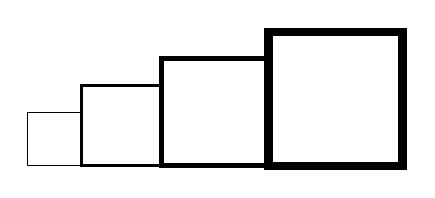
\begin{tikzpicture}[x = 0.017cm, y = 0.017cm]
	\foreach \c in {0,...,3} {
		\draw[line width = \c pt,shift = {(30*\c+10*\c*\c,0)}] (0,0) -- (40+20*\c,0) -- (40+20*\c,40+20*\c) -- (0 , 40+20*\c) -- cycle;  }
	\end{tikzpicture}
	
	\vspace{8mm}
	
	\begin{scratch}
		\blockinit{quand ~\greenflag ~est cliqué}
		\blockmove{aller à x : \ovalnum{--200} y : \ovalnum{0}}
		\blockmove{s'orienter à \ovalnum{90 ~\selectarrownum}}
		\blockpen{effacer tout}
		\blockpen{mettre la taille du stylo à \ovalnum{1}}
		\blockvariable{mettre \selectmenu{côté} à \ovalnum{40}}
		\blockrepeat{répéter \ovalnum{4} fois}
		{
			\blockmoreblocks{carré}
			\blockmove{avancer de \ovaloperator{\ovalvariable{côté} + \ovalnum{30}}}
			\blockvariable{ajouter à \selectmenu{côté} \ovalnum{20}}
		}
	\end{scratch}

\vspace{3mm}

\textbf{Pour rappel : le bloc carré}
\begin{scratch}
	\initmoreblocks{définir \namemoreblocks{carré}}
	\blockpen{stylo en position d'écriture}
	\blockrepeat{répéter \ovalnum4 fois}
	{\blockmove{avancer de \ovalvariable{coté}}
		\blockmove{tourner \turnleft{} de \ovalnum{90} degrés}
	}
	\blockpen{relever le stylo}
\end{scratch}
	\end{center}
\end{minipage}


